\documentclass[]{article}
\usepackage{geometry}   % my added package "geometry"
\geometry{letterpaper,tmargin=1in,bmargin=1in,lmargin=2.2cm,rmargin=2.2cm}
\usepackage[colorlinks,bookmarksopen,bookmarksnumbered,
citecolor=green,urlcolor=red]{hyperref}
\hypersetup{pdfauthor={Name}}
%%%%%%%%%%%%%%%%%%%%%%%%%%%%%%%%%%%%%%%%%%%%%%%%%%%%%%%%%%%%%%%%%%%%%%%%%
%\usepackage{graphicx}
\usepackage{graphics}
\usepackage{epsfig}
\usepackage{epstopdf}
\usepackage{amsfonts}
\usepackage{amssymb}
\usepackage{booktabs}
\usepackage{color,soul}
%%%%%%%%%%%%%%%%%%%%%%%%%%%%%%%%%%%%%%%%%%%%%%%%%%%%%%%%%%%%%%%%%
\usepackage{amsmath}
\usepackage{cleveref}
%\usepackage[fleqn]{amsmath}
\usepackage{lineno}
\usepackage{tikz}
\usepackage{standalone}
\usetikzlibrary{calc,patterns,arrows.meta,shapes.arrows,intersections,positioning}
\usetikzlibrary{decorations.pathmorphing,backgrounds,fit,petri}
\usepackage[percent]{overpic}
%%%%%%%%%%%%%%%%%%%%%%%%%%%%%%%%%%%%%%%%%%%%%%%%%%%%%%%%%%%%%%%%%
\usepackage{xcolor}
\usepackage{listings}
\lstset { %
	language=C++,
	backgroundcolor=\color{blue!5}, % set backgroundcolor
	basicstyle=\footnotesize\color{black},% basic font settingbasicstyle=\ttfamily\color{black}
	keywordstyle=\color{red},
	commentstyle=\color{violet},
	stringstyle=\color{blue},
	xleftmargin=2em,
	frame=single,
	framexleftmargin=2em,
	numbers=left,
	numberstyle=\tiny,
	numbersep=8pt,
}
%%%%%%%%%%%%%%%%%%%%%%%%%%%%%%%%%%%%%%%%%%%%%%%%%%%%%%%%%%%%%%%%%
\renewcommand\thesubsection{\thesection\Alph{subsection}}
%%%%%%%%%%%%%%%%%%%%%%%%%%%%%%%%%%%%%%%%%%%%%%%%%%%%%%%%%%%%%%%%%
\renewcommand\lstlistingname{Header}
\renewcommand\lstlistlistingname{Header}
%%%%%%%%%%%%%%%%%%%%%%%%%%%%%%%%%%%%%%%%%%%%%%%%%%%%%%%%%%%%%%%%%%%%
%opening
\begin{document}
\title{HiperLife Tutorial: Thermal Conduction}
\author{LaCàN}
\maketitle

\linenumbers

\section{Problem Definition} \label{sec: pd} 
Thermal conduction is the diffusion of thermal energy within one material or between materials in contact. Here we consider an  example of time-dependent linear problem. Consider the transient heat conduction equation \cite{reddy2014introduction}

\begin{equation}\label{eq1}
	\begin{aligned}
		 \frac{\partial \theta}{\partial t} - (\frac{\partial^2 \theta}{\partial x^2}+\frac{\partial^2 \theta}{\partial y^2}) = 1
	\end{aligned}
\end{equation}

where $\theta$ is the non-dimensional temperature in the doamin of $\Omega=[-1,-1]\times[1,1]$, which its
boundary condition is $\theta = 0$ on $\Gamma$ for $t > 0$ (see Figure \ref{fig_SB}). The initial
condition is that $\theta(x, y, 0) = 0$. We wish to find the temperature field inside the domain for
$t > 0$.
\begin{figure}[htbp]
	\centering
	
\documentclass[preprint,12pt,a4]{standalone}
\usepackage{geometry}   % my added package "geometry"
\geometry{letterpaper,tmargin=1in,bmargin=1in,lmargin=2.5cm,rmargin=2.5cm}
\usepackage{tikz}
\usetikzlibrary{calc,patterns,arrows.meta,shapes.arrows,intersections,positioning}
\usetikzlibrary{decorations.pathmorphing,backgrounds,fit,petri}
\usepackage{standalone}
\begin{document}
	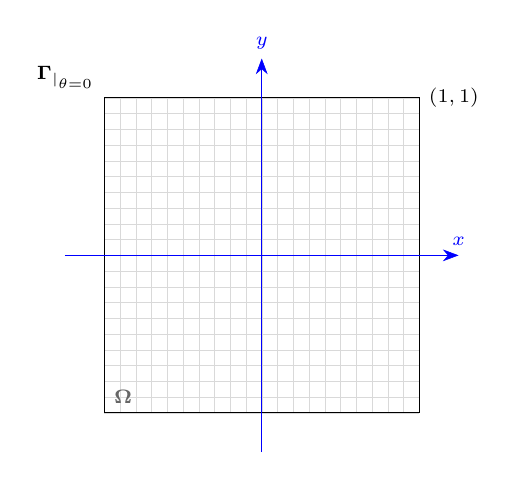
\begin{tikzpicture} [{place/.style={rectangle,draw=blue!50,fill=blue!20,ultra thin,inner sep=0.8mm}},{place2/.style={circle,draw=black!50,ultra thin,inner sep=0.8mm}},{linest/.style={color=gray,ultra thin}}]
	%%coordinates of corners of Beam
	\coordinate (A) at (-2.0,-2.0);
	\coordinate (B) at (2.0,-2.0);
	\coordinate (D) at (2.0,2.0);
	\coordinate (E) at (-2.0,2.0);
	

	%%mesh
	\draw [line width=0.1pt,gray!30,step=2mm](A) grid (D);
	%%Beam	
	\draw [color=black](A)node [above right,color = black!60,font=\scriptsize] {$\boldsymbol{\Omega}$} -- (B)--(D)node [right,color = black,font=\scriptsize] {$(1,1)$} --(E)node [above left,color = black,font=\scriptsize] {$\boldsymbol{\Gamma}_{|_{\theta=0}}$} --(A);
	
	%%axes
	\draw [-{Stealth[length=2mm]},help lines,blue] ($(A)-(0.5,-2)$) -> ($(B)+(0.5,2)$) node [above,color = blue,font=\scriptsize] {$x$};
		\draw [-{Stealth[length=2mm]}, help lines,blue] ($(A)+(2.0,-0.5)$) -> ($(D)+(-2,0.5)$) node [above,color = blue,font=\scriptsize] {$y$};

	\end{tikzpicture}
\end{document}
	\caption{Illustration of the domain of transient heat transfer problem.}
	\label{fig_SB}
\end{figure}

The paramteres of problem are listed as
\begin{equation}\label{eq2}
	\begin{aligned}
		&\text{space discretiziation step}= \Delta x = \Delta y = 0.1, \\
		&\text{time discretiziation step}= \Delta T = 0.05, \\
		&\text{initial distribution}= f(x,y) = 0.0\\
	\end{aligned}
\end{equation}

Note that the most commonly used method for solving parabolic equation like $([C_e ]\{\dot{u}\} + [K_e]\{u_e \} = \{F_e \})$, is the $\alpha$-family of approximation, in which a weighted average of the time derivative of a dependent variable is approximated at two consecutive time steps by linear interpolation of the values of the variable at the two steps:
\begin{equation}\label{eq3}
	\begin{aligned}
		(1 - \alpha)\{\dot{u}\}^n + \alpha\{\dot{u}\}^{n+1} \approx \frac{\{u\}^{n+1} - \{u\}^n}{t^{n+1} - t^{n}}  \quad \text{for} \quad 0 \leq \alpha \leq 1
	\end{aligned}
\end{equation}
We choose a uniform mesh of $16 \times 16$ to model the domain, and investigate the stability and accuracy of forward method $(\alpha = 0.0)$, Crank-Nicolson $(\alpha = 0.5)$ and backward difference $(\alpha = 1.0)$.
\section{Weak Form} \label{sec: WF}
By considering $\Delta t = t^{n+1} - t^{n}$, and substituting $u$ with our temperature field, Eq. (\ref{eq3})  takes the following form
\begin{equation}\label{eq4}
	\begin{aligned}
	\{\theta\}^{n+1} = \{\theta\}^n + \Delta t(1 - \alpha)\{\theta_t\}^n + \Delta t\alpha\{\theta_t\}^{n+1}
	\end{aligned}
\end{equation}
The time derivatives of $\theta$ on the right hand side of this equation can be calculated from Eq. (\ref{eq1}) for each step, like this 
\begin{equation}\label{eq5}
	\begin{aligned}
		\{\theta_t\}^{n+1} &= 1 + \nabla^2 \{\theta\}^{n+1}\thinspace,\\
		\{\theta_t\}^{n} &= 1 + \nabla^2 \{\theta\}^{n}\thinspace. \\
	\end{aligned}
\end{equation}
combining these two equations gives us
\begin{equation}\label{eq6}
	\begin{aligned}
		\{\theta\}^{n+1} -\Delta t\alpha[1 + \nabla^2 \{\theta\}^{n+1}] - \{\theta\}^n - \Delta t(1 - \alpha)[1 + \nabla^2 \{\theta\}^{n}]=0\thinspace .
	\end{aligned}
\end{equation}
The variation formulation of our model problem can be introduced as find $\theta \in V$ such that
\begin{equation}\label{eq7}
	\begin{aligned}
		\mathcal{F}(\theta;v) = 0 \quad \forall v \in \hat{V}\thinspace.
	\end{aligned}
\end{equation}
where
\begin{equation}\label{eq8}
	\begin{aligned}
		\mathcal{F}(\theta; v) =\int_{\Omega} v\{\theta\}^{n+1} -\Delta t\alpha v[1+\nabla^2\{ \theta\}^{n+1}] - v\{\theta\}^n - \Delta t(1 - \alpha)v[1+\nabla^2\{\theta\}^{n}]\ \mathrm{d}\Omega \thinspace .
	\end{aligned}
\end{equation}
and
\begin{equation}\label{eq9}
	\begin{aligned}
		\hat{V} &= \{v \in H^1(\Omega) : v = 0 \text{ on } \Gamma\}, \\
		V &= \{v \in H^1(\Omega) : v = 0 \text{ on } \Gamma\}\thinspace.
	\end{aligned}
\end{equation}
Considering  $\boldsymbol{\theta} = \sum \phi_j \theta_j$, and applying integration by part, and also boundary condition, the weak form takes the following form
\begin{equation}\label{eq7}
	\begin{aligned}
		\mathcal{F}(\theta; v)=\int_{\Omega} \phi_i \phi_j\{\theta\}^{n+1}_j - \Delta t \alpha [\phi_i - \nabla \phi_i (\nabla \phi_j\{\theta\}^{n+1}_j)] \mathrm{d} \Omega - \int_{\Omega} \phi_i\theta^{n} + \Delta t (1-\alpha) [\phi_i -\nabla \phi_i \nabla\theta^n ] \mathrm{d} \Omega\thinspace.
	\end{aligned}
\end{equation}
Lets rewrite this equation for known and unkown variables. the final formulation need for implementation takes the form of
\begin{equation}\label{eq8}
	\begin{aligned}[b]
		\mathcal{F}(\theta; v)=\int [\phi_i\phi_j + \Delta t \alpha\nabla\phi_i\nabla\phi_j]\{\theta\}^{n+1} \mathrm{d} \Omega - \int  [\phi_i\theta^{n}+\Delta t \alpha \phi_i + \Delta t (1-\alpha) (\phi_i - \nabla \phi_i \nabla\theta^n)]\mathrm{d} \Omega\thinspace.
	\end{aligned}
\end{equation}
So the final formulation need for implementation takes the form of
\begin{equation}\label{eq9}
	\begin{aligned}[b]
		Bk (i) &= jac \times [\phi_i \theta^n + \Delta t  \phi_i - \Delta t (1-\alpha)(\nabla \phi_i \cdot \nabla \theta^n)] \\
		Ak (i,j) &=  jac \times [\phi_i\phi_j + \Delta t \alpha(\frac{\partial \phi_i}{\partial x}
		\frac{\partial \phi_j}{\partial x} + \frac{\partial \phi_j}{\partial y} 
		\frac{\partial \phi_j}{\partial y})]  
	\end{aligned}
\end{equation}
\section{Implementation} \label{sec: imp}
In this section, we present the implementation of our solution in the Hiperlife. The program is divided into three separate files, main part which we create our problem by the Hiperlife headers, auxiliary header where we introduce parameters and declare defined functions, and at last auxiliary file, where we define some functions which provide required matrices like the Jacobian.
\subsubsection{HeatTransfer.cpp} \label{sec: m.cpp}
\nolinenumbers
\begin{lstlisting}
/* Heat Transfer conduction*/
// cpp headers
#include <iostream>
#include <fstream>
#include <cmath>
	
// hiperlife headers
#include "hl_Core.h"
#include "hl_Parser.h"
#include "hl_TypeDefs.h"  
#include "hl_DOFsHandler.h"
#include "hl_HiPerProblem.h"
#include "hl_FillStructure.h"
#include "hl_ParamStructure.h"
#include "hl_DistributedMesh.h" 
#include "hl_StructMeshGenerator.h" 
#include "hl_GlobalBasisFunctions.h"
#include "hl_NonlinearSolver_NewtonRaphson.h"
#include "hl_LinearSolver_Iterative_AztecOO.h"
	
// Header to auxiliary functions
#include "AuxHeatTransfer.h"
	
// -------------------------------------------------------------------//
// -----------------    MAIN FUNCTION     ----------------------------//
// -------------------------------------------------------------------//
	
int main(int argc, char** argv)
{
	using namespace std;
	using namespace hiperlife;
	using namespace hiperlife::Tensor;
		
	// ---------------------------------------------------------------//
	// *****                 INITIALIZATION                    *****  //
	// ---------------------------------------------------------------//
		
	// Initialize MPI
	hiperlife::Init(argc, argv);
		
	// ---------------------------------------------------------------//
	/// *****                   DATA INPUT                      *****///
	// ---------------------------------------------------------------//
		
	// Put parameters in the user structure
	SmartPtr<ParamStructure> paramStr = CreateParamStructure<HeatParams>();
		
	// Data
	paramStr->setRealParameter(HeatParams::delta_t, 0.05);
	paramStr->setRealParameter(HeatParams::alpha, 0.5);
	double delta_t = paramStr->getRealParameter(HeatParams::delta_t);
	double alpha = paramStr->getRealParameter(HeatParams::alpha);
		
	// ---------------------------------------------------------------//
	/// *****                   MESH CREATION                   *****///
	// ---------------------------------------------------------------//
		
	// Create a line structured mesh       
	SmartPtr<StructMeshGenerator> structMesh = Create<StructMeshGenerator>();
	structMesh->setNDim(3);
	structMesh->setBasisFuncType(BasisFuncType::Lagrangian);
	structMesh->setBasisFuncOrder(1);
	structMesh->setElemType(ElemType::Square);
	structMesh->genRectangle(16, 16, 2.0, 2.0);
	structMesh->translateX(-1.0);
	structMesh->translateY(-1.0);
		
	// Distributed mesh
	SmartPtr<DistributedMesh> disMesh = Create<DistributedMesh>();
	disMesh->setMesh(structMesh);
	disMesh->setBalanceMesh(true);
	disMesh->setElementLocatorEngine(ElementLocatorEngine::BoundingVolumeHierarchy);
	disMesh->Update();
	disMesh->printFileLegacyVtk("mesh");
		
	// ---------------------------------------------------------------//
	/// *****               DOFsHANDLER CREATION                *****///
	// ---------------------------------------------------------------//
		
	// DOFHandler
	SmartPtr<DOFsHandler> dofHand = Create<DOFsHandler>(disMesh);
	dofHand->setNameTag("dofHand");
	dofHand->setNumDOFs(1);
	dofHand->setDOFs({"theta"});
	dofHand->Update();
	// ------------------ Initial conditions------------------------ //
	//---------------------------------------------------------------//
	double f;
	for (int i = 0; i < disMesh->loc_nPts(); i++)
	{
		// Coordinate
		double x = dofHand->mesh->nodeCoord(i, 0, hiperlife::IndexType::Local);
		f = 0.0 * x;
		// Initial condition
		dofHand->nodeDOFs->setValue("theta", i, IndexType::Local, f);
	}
		
	// Update 
	dofHand->UpdateGhosts();
	// ------------------ Boundary conditions------------------------ //
	//---------------------------------------------------------------//
	dofHand->setBoundaryCondition(0, MAxis::Xmin, 0.0);
	dofHand->setBoundaryCondition(0, MAxis::Xmax, 0.0);
		
	dofHand->setBoundaryCondition(0, MAxis::Ymin, 0.0);
	dofHand->setBoundaryCondition(0, MAxis::Ymax, 0.0);
	// Update 
	dofHand->UpdateGhosts();
	// ---------------------------------------------------------------//
	/// *****               HIPERPROBLEM CREATION               *****///
	// ---------------------------------------------------------------//
		
	SmartPtr<HiPerProblem> hiperProbl = Create<HiPerProblem>();
	hiperProbl->setParameterStructure(paramStr);
	hiperProbl->setDOFsHandlers({dofHand});
	hiperProbl->setIntegration("Integ", {"dofHand"});
	hiperProbl->setCubatureGauss("Integ", 4);
	hiperProbl->setElementFillings("Integ", LS);
	hiperProbl->Update();
		
	// ---------------------------------------------------------------//
	/// *****                  SOLVER CREATION                  *****///
	// ---------------------------------------------------------------//
	SmartPtr<AztecOOIterativeLinearSolver> solver=Create<AztecOOIterativeLinearSolver>();
	solver->setHiPerProblem(hiperProbl);
	solver->setTolerance(1.E-8);
	solver->setMaxNumIterations(500);
	solver->setSolver(AztecOOIterativeLinearSolver::Solver::Gmres);
	solver->setPreconditioner(AztecOOIterativeLinearSolver::Preconditioner::None);
	solver->setDefaultParameters();
	solver->setVerbosity(AztecOOIterativeLinearSolver::Verbosity::High);
	solver->Update();
	// ---------------------------------------------------------------//
	/// *****                SOLVE HIPERPROBLEM                 *****///
	// ---------------------------------------------------------------//
		
	// Time params
	double maxTime  = 1.05;
	double maxTimeSteps = 1000;
		
	// Initialize
	double time{delta_t};
	int timeStep{1};
		
	// Time loops
	while ((time <= maxTime) && (timeStep < maxTimeSteps))
	{
		// initial value for theta
		dofHand->nodeDOFs0->setValue(dofHand->nodeDOFs);
		// Update 
		dofHand->UpdateGhosts();
		// time step info
		if (hiperProbl->myRank() == 0)
		{
			cout<<endl<<"TS:"<<timeStep<<"dt:"<<delta_t<<"|"
			<<"Time"<<time<<"of time"<<maxTime<<endl; 
		}
		// ------------------- Linear solver ------------------------ //
		// ---------------------------------------------------------- //
		bool converged = solver->solve();
		if (!converged)
		{
			throw runtime_error("Error: Linear solver does not converge.");
			break;
		}
		// Update solution
		solver->UpdateSolution(); 
		// Update time variables
		timeStep ++;
		time += delta_t;
		// -------------------- Post Proccessing  --------------------//
		// -----------------------------------------------------------//
		string solName = "Conduct." + to_string(timeStep);
		dofHand->printFileLegacyVtk(solName,true);
	}
		
	hiperlife::Finalize();
	return 0;
}	
\end{lstlisting}
\subsubsection{AuxHeatTransfer.h} \label{sec: a.h}
\begin{lstlisting}
#ifndef AUXHeat_H
#define AUXHeat_H

// C headers
#include <iostream>

// hiperlife headers
#include "hl_Core.h"
#include "hl_Parser.h"
#include "hl_TypeDefs.h"  
#include "hl_DOFsHandler.h"
#include "hl_HiPerProblem.h"
#include "hl_FillStructure.h"
#include "hl_ParamStructure.h"
#include "hl_DistributedMesh.h" 
#include "hl_StructMeshGenerator.h" 
#include "hl_GlobalBasisFunctions.h"
#include "hl_NonlinearSolver_NewtonRaphson.h"
#include "hl_LinearSolver_Iterative_AztecOO.h"

// time parameters
// alpha = 0.0: forward;        delta_t = 0.001
// alpha = 0.5: crank-nicolson; delta_t = 0.05
// alpha = 1.0: backward;       delta_t = 0.05

struct HeatParams
{
	enum RealParameters
	{
		delta_t,
		alpha,
	};
	HL_PARAMETER_LIST DefaultValues
	{
		{"delta_t,", 0.05},
		{"alpha,", 0.5},
	};
};

void LS(hiperlife::FillStructure& fillStr);

#endif
\end{lstlisting}
\subsubsection{AuxHeatTransfer.cpp} \label{sec: a.cpp}
\begin{lstlisting}
// Header to auxiliary functions
#include "AuxHeatTransfer.h"

// Hiperlife headers
#include "hl_Core.h"
#include "hl_ParamStructure.h"
#include "hl_Parser.h"
#include "hl_TypeDefs.h"                                                                         
#include "hl_GlobalBasisFunctions.h"                             
#include "hl_StructMeshGenerator.h"                                                                             
#include "hl_DistributedMesh.h"                                           
#include "hl_FillStructure.h"                                             
#include "hl_DOFsHandler.h"          
#include "hl_HiPerProblem.h"         
#include "hl_LinearSolver_Iterative_AztecOO.h"
#include "hl_NonlinearSolver_NewtonRaphson.h"

using namespace std;
using namespace hiperlife;
using namespace hiperlife::Tensor;


// Conduction

void LS(hiperlife::FillStructure& fillStr)
{
	double alpha  = fillStr.getRealParameter(HeatParams::alpha);
	double delta_t = fillStr.getRealParameter(HeatParams::delta_t);
	
	//--------------------------------------------------------------------------//
	// --------------------------- INPUT DATA ----------------------------------//
	//--------------------------------------------------------------------------//
	
	// Dimensions
	SubFillStructure& subFill = fillStr["dofHand"];
	int nDOFs = subFill.numDOFs;                                        
	int eNN   = subFill.eNN;                                           
	int nDim  = subFill.nDim;                                        
	int pDim  = subFill.pDim;
	// Nodal values at Gauss points
	wrapper<double,1> nborDOFs(subFill.nborDOFs.data(),eNN);
	wrapper<double,1> nborDOFs0(subFill.nborDOFs0.data(),eNN);
	
	// Shape functions and derivatives at Gauss points
	double jac; 
	wrapper<double,1>  bf(subFill.nborBFs(), eNN);
	tensor<double,2> Dbf(eNN,pDim); 
	GlobalBasisFunctions::gradients(Dbf, jac, subFill);
	
	//--------------------------------------------------------------------------//
	// ---------------------------- OUTPUT DATA --------------------------------//
	//--------------------------------------------------------------------------//
	wrapper<double,2> Ak(fillStr.Ak(0, 0).data(), eNN, eNN);
	wrapper<double,1> Bk(fillStr.Bk(0).data(),eNN);
	
	//--------------------------------------------------------------------------//
	// ---------------------------- KNOWN VARIABLES ----------------------------//
	//--------------------------------------------------------------------------//
	
	// Temperature
	double theta = bf*nborDOFs0;
	// Temperature Gradient
	tensor<double,1> grad_theta(pDim);
	for (int i = 0; i < eNN; i++)
	{
		for (int d = 0; d < pDim; d++)
		grad_theta(d) += Dbf(i,d)*nborDOFs0(i); 
	}
	
	//--------------------------------------------------------------------------//
	//---------------------------- EQUATIONS -----------------------------------//
	//--------------------------------------------------------------------------// 
	for (int i = 0; i < eNN; i++)            //i for basis functions
	{
		// (gradient of the basis function) *  (gradient of u)
		double dotdg{};
		for (int d = 0; d < pDim; d++)
		dotdg += Dbf(i,d)*grad_theta(d);
		// Fill RHS
		Bk(i) += jac * (bf(i)*theta + delta_t*bf(i) - delta_t*(1.0-alpha)*dotdg);
		for (int j = 0; j < eNN; j++)       //j for variable.
		{
			// (gradient of the basis function)*(gradient of the basis function)
			double dotdd{};
			for (int d = 0; d < pDim; d++)
			dotdd += Dbf(i,d)*Dbf(j,d);
			
			// Fill matrix
			Ak(i,j) += jac * (bf(i)*bf(j) + delta_t*alpha*dotdd);
		}
	}
}

\end{lstlisting}
\section{Results} \label{sec: rst}
In this section, we present the results of our solution. Table \ref{tab1} shows the evolution of $\theta(0, 0, t)$ in different time approximation scheme. These values is presented for Crank-Nicholson scheme in Figure \ref{fig_Rs}. The contour demonstration of temperature in the whole domain at $t=1$ is also shown in Figure \ref{fig_Rs2}. 
\begin{table}
	\caption{Evolution of $\theta(0, 0, t)$ with various time
		approximation schemes.}
	\label{tab1}
	\begin{center}
		\begin{tabular}{|c| c| c| c|} 
			\hline
			Time & Crank-Nocholson & Backward Difference & Forward Difference\\ [0.7ex] 
			\hline\hline
			0.05 & 0.0497 & 0.0480 & 0.0500\\  [0.2ex] 
			\hline
			0.2 & 0.1740 & 0.1612 & 0.1737\\ [0.2ex] 
			\hline
			0.4 & 0.2506 & 0.2395 & 0.2503\\ [0.2ex] 
			\hline
			0.6 & 0.2790 & 0.2724 & 0.2788\\ [0.2ex] 
			\hline
			0.8 & 0.2895 & 0.2860 & 0.2894\\ [0.2ex] 
			\hline
			1.0 & 0.2933 & 0.2916 & 0.2933\\ [0.2ex] 
			\hline
		\end{tabular}
	\end{center}
\end{table}
\begin{figure}[htbp]
	\centering
	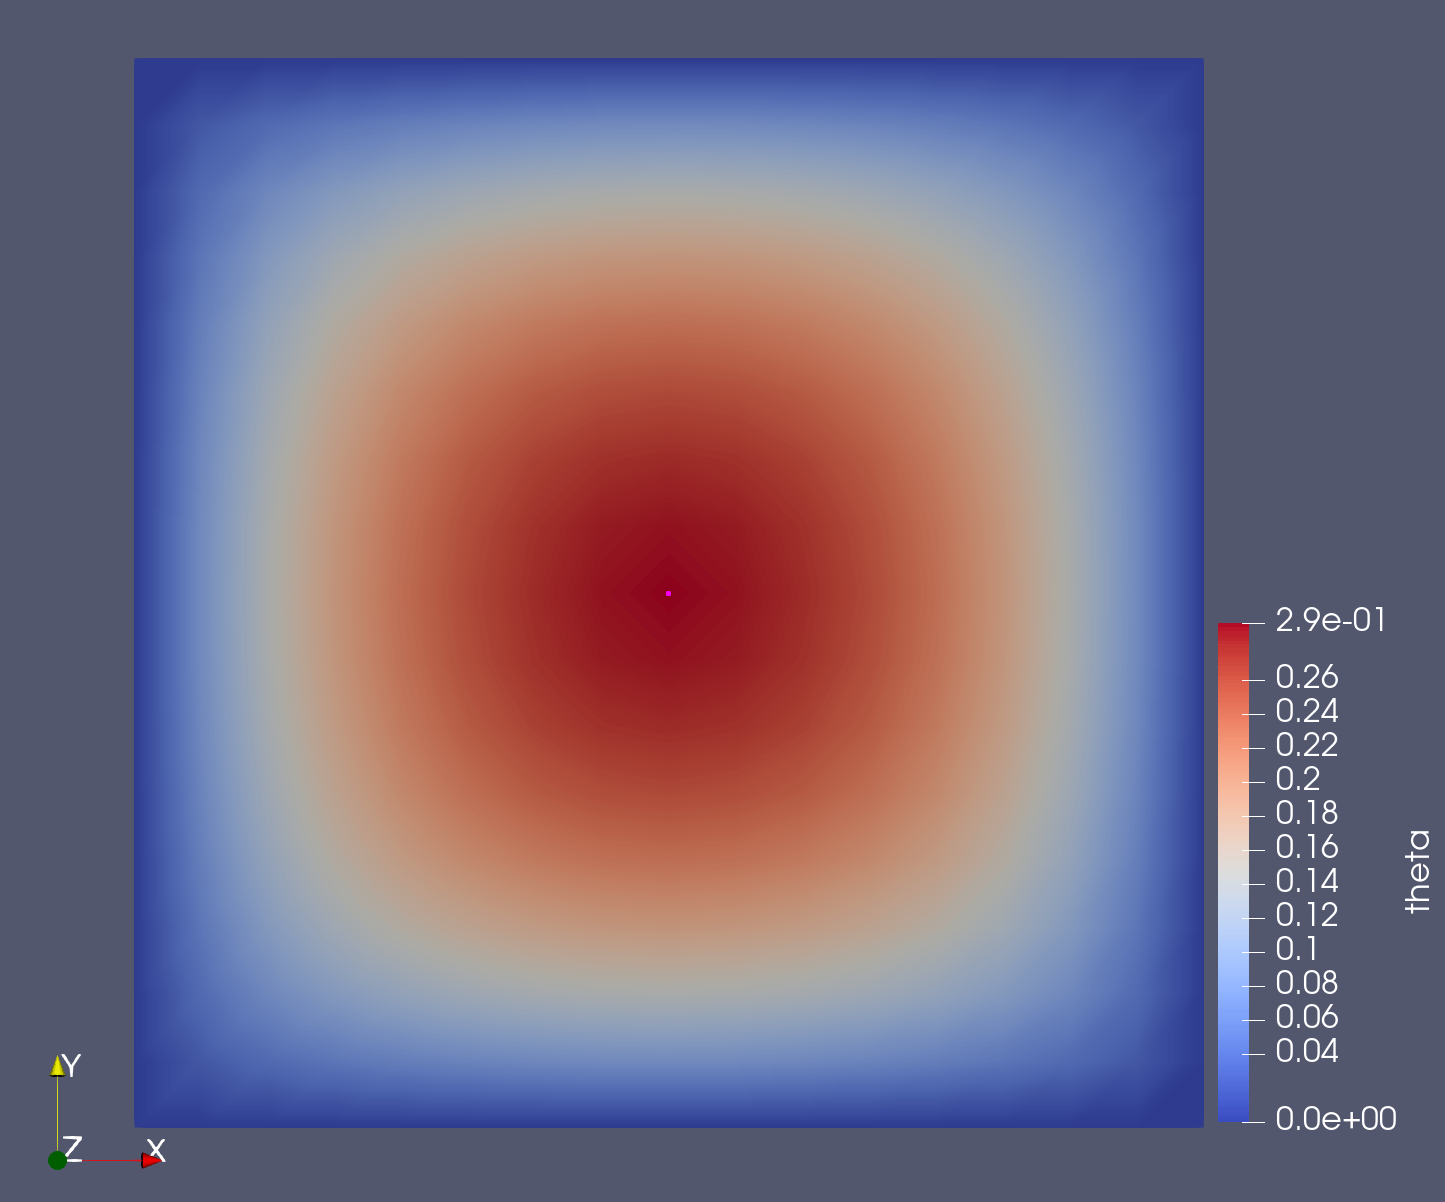
\includegraphics[width=0.6\textwidth]{Figures/result1.png}
	\caption{$\theta(x, y, 1.0)$}
	\label{fig_Rs}
\end{figure}
\begin{figure}[htbp]
	\centering
	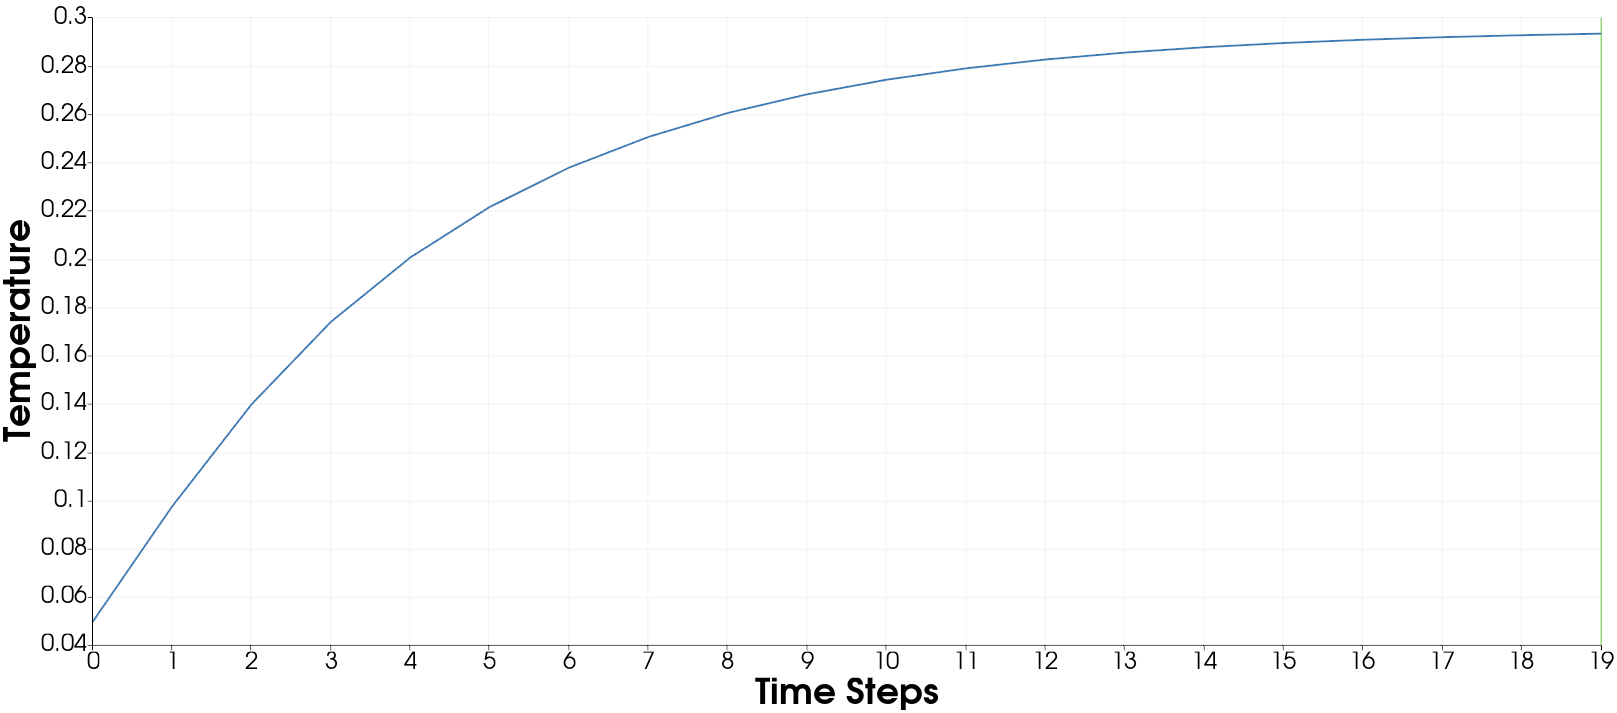
\includegraphics[width=0.6\textwidth]{Figures/result2.png}
	\caption{Evolution of $\theta(0, 0, t)$ for time steps.}
	\label{fig_Rs2}
\end{figure}
\bibliographystyle{unsrt}
\bibliography{ref}
\end{document}
